\documentclass[tikz,border=5pt]{standalone}
\usepackage{amsmath}
\usetikzlibrary{arrows.meta,positioning,calc}

\definecolor{siteaccent}{RGB}{54,117,138}
\definecolor{sitelight}{RGB}{238,245,247}
\definecolor{siteborder}{RGB}{190,211,218}
\definecolor{sitetext}{RGB}{32,39,43}
\definecolor{sitemuted}{RGB}{102,116,123}

\tikzset{
  block/.style={draw=siteborder, fill=sitelight, rounded corners=2pt,
    minimum width=24mm, minimum height=12mm, align=center, inner xsep=4pt, text=sitetext},
  route/.style={draw=siteaccent, fill=white, rounded corners=2pt,
    minimum width=27mm, minimum height=12mm, align=center, inner xsep=4pt, text=sitetext},
  flow/.style={-{Latex[length=2.2mm]}, semithick, draw=siteaccent}
}

\begin{document}
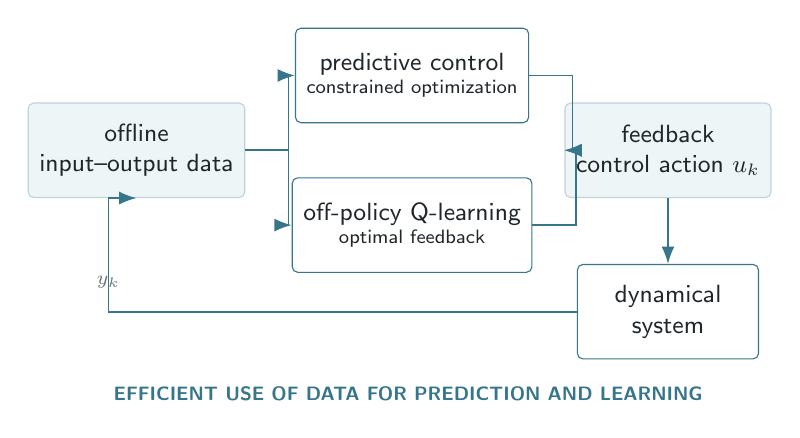
\begin{tikzpicture}[font=\sffamily\small]
  \node[block] (data) at (0,0.8) {offline\\input--output data};
  \node[route] (predictive) at (3.5,1.75) {predictive control\\[-1mm]\scriptsize constrained optimization};
  \node[route] (learning) at (3.5,-0.15) {off-policy Q-learning\\[-1mm]\scriptsize optimal feedback};
  \node[block] (action) at (6.75,0.8) {feedback\\control action $u_k$};
  \node[route, minimum width=23mm] (plant) at (6.75,-1.25) {dynamical\\system};

  \draw[flow] (data.east) -- ++(0.55,0) |- (predictive.west);
  \draw[flow] (data.east) -- ++(0.55,0) |- (learning.west);
  \draw[flow] (predictive.east) -- ++(0.55,0) |- (action.west);
  \draw[flow] (learning.east) -- ++(0.55,0) |- (action.west);
  \draw[flow] (action) -- (plant);
  \draw[flow] (plant.west) -- ++(-5.95,0) |- node[pos=0.2, below, text=sitemuted, font=\scriptsize] {$y_k$} (data.south);

  \node[anchor=north, text=siteaccent, font=\sffamily\scriptsize\bfseries]
    at (3.45,-2.08) {EFFICIENT USE OF DATA FOR PREDICTION AND LEARNING};
\end{tikzpicture}
\end{document}
